\captionsetup[subfigure]{justification=justified,singlelinecheck=false}

\begin{figure*}[t]
  \centering
  \begin{subfigure}[t]{0.35\linewidth}
    \centering
    \caption{\mnist \MNISTNET (GPU)}
    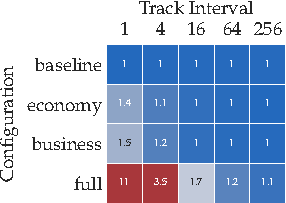
\includegraphics{../repos/cockpit-paper/fig/01_benchmark/output/fig_grid/benchmark_mnist_logreg_cuda_app_thesis-wide}
    \label{cockpit::fig:app_benchmark_configurations_cuda-mnist_logreg}
  \end{subfigure}
  \hspace{0.1\linewidth}
  \begin{subfigure}[t]{0.35\linewidth}
    \centering
    \caption{\mnist \mlp (GPU)}
    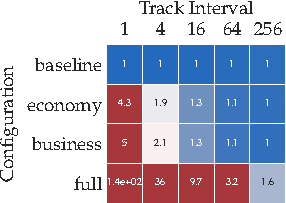
\includegraphics{../repos/cockpit-paper/fig/01_benchmark/output/fig_grid/benchmark_mnist_mlp_cuda_app_thesis-wide}
    \label{cockpit::fig:app_benchmark_configurations_cuda-mnist_mlp}
  \end{subfigure}
  \begin{subfigure}[t]{0.35\linewidth}
    \centering
    \caption{\cifarten \threecthreed (GPU)}
    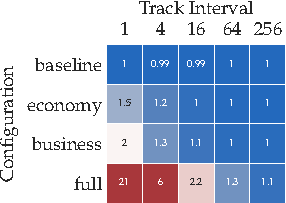
\includegraphics{../repos/cockpit-paper/fig/01_benchmark/output/fig_grid/benchmark_cifar10_3c3d_cuda_app_thesis-wide}
    \label{cockpit::fig:app_benchmark_configurations_cuda-cifar}
  \end{subfigure}
  \hspace{0.1\linewidth}
  \begin{subfigure}[t]{0.35\linewidth}
    \centering
    \caption{\fmnist \twoctwod (GPU)}
    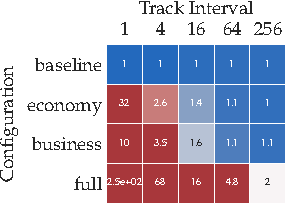
\includegraphics{../repos/cockpit-paper/fig/01_benchmark/output/fig_grid/benchmark_fmnist_2c2d_cuda_app_thesis-wide}
    \label{cockpit::fig:app_benchmark_configurations_cuda-fmnist}
  \end{subfigure}
  \caption{\textbf{Overhead of \cockpittitle configurations on GPU for four
      different problems with varying tracking interval.} Color bar is the same
    as in \autoref{cockpit::fig:benchmark}.}
  \label{cockpit::fig:app_benchmark_configurations_cuda}
\end{figure*}

\captionsetup[subfigure]{justification=centering, singlelinecheck=true}

%%% Local Variables:
%%% mode: latex
%%% TeX-master: "../../../thesis"
%%% End:
